%\begin{document}
\documentclass[a4paper,12pt]{article}
\usepackage{indentfirst}%paragrafo no primeiro tb
\usepackage[english,brazil]{babel}
\usepackage[utf8]{inputenc}
\usepackage{amsmath}
\usepackage[mathcal]{euscript}
\usepackage{graphicx}
\usepackage{fancyhdr}
\usepackage{url}
\renewcommand{\baselinestretch}{1.5}
\usepackage{setspace}%%%% pacote para espaço duplo
\usepackage{titling}
\usepackage{geometry}
\usepackage{amsmath}
\usepackage{amssymb}
%\usepackage{subfigure}
\usepackage{multirow}
\usepackage[table]{xcolor}
\usepackage{fullpage}
\usepackage[backend=bibtex,style=ieee,sorting=none]{biblatex}
\usepackage{subfig}
\usepackage[shortlabels]{enumitem}
\addbibresource{refs.bib}



\newcolumntype{C}{>{\centering\arraybackslash}p{1em}}

% FAPESP pede "tipo equivalente a Times New Roman"
% Acho que na verdade eles só estão preocupados com o tamanho da fonte
% A diferença entre a fonte padrão do LaTeX e times é pequena
%\usepackage{times}

\title{\textbf{Relatório Final de Atividades
\\
\vspace{20px}
Controle de Estabilização de Caminhada de Robô Humanoide
}\\
\vspace{20px}
\normalsize \textbf{Bolsa de Iniciação Científica 
2020/04559-6}\\
\normalsize \textbf{Período relatado: 10/12/2020 a 30/06/2021}\\
\normalsize \textbf{Período de vigência: 01/07/2020 a 30/06/2021}\\
 \textbf{Instituto Tecnológico de Aeronáutica -- ITA}
 }






%%%%


\author{\textbf{Aluno:} Reynaldo Santos de Lima\\
\textbf{Orientador:} Marcos Ricardo Omena de Albuquerque Maximo\\
 } %\\

%%%%%%%

\date{\today}
% ADD THE FOLLOWING COUPLE LINES INTO YOUR PREAMBLE
\let\OLDthebibliography\thebibliography
\renewcommand\thebibliography[1]{
  \OLDthebibliography{#1}
  \setlength{\parskip}{0pt}
  \setlength{\itemsep}{0pt plus 0.3ex}
}


\begin{document}
\maketitle
%\newpage
%\maketitle
\thispagestyle{empty}
\selectlanguage{brazil}
\begin{abstract}
Neste trabalho estudam-se adaptações em algoritmos de estabilização de caminhada em robô humanoide de baixo custo (ITAndroids Chape 1ª e 2ª gerações). Esse trabalho será realizado no  Laboratório de Sistemas Computacionais Autônomos (LAB-SCA), onde desenvolvem-se robôs humanoides. São apresentados aspectos importantes do modelo em baixo nível do controle, com a equação do manipulador ilustrando a dinâmica utilizada para cada plano considerado no controle de estabilização (coronal e sagital). Dá-se destaque à interface prática das diferentes ferramentas utilizadas no desenvolvimento e projeto dos ganhos do controlador, bem como as melhorias adotadas neste trabalho com o objetivo de tornar o código humanoide mais seguro, mais modularizado e de manutenibilidade maior. 

\noindent \textbf{Palavras chaves:} Caminhada de robôs humanoides, Controle, Robótica.


%%%
\end{abstract}
\newpage

\tableofcontents

\newpage
%%%%%
\doublespacing
%%%%%%
\section{Resumo do plano inicial}\label{sec:plano}

O plano inicial, do trabalho de 12 meses, com início em julho de 2020, dividido em execução nas atividades listadas a seguir:
\begin{enumerate}[A]
\item{Estudo introdutório da matéria de controle;}
\item{Estudo sobre algoritmos de otimização;}
\item{Estudo sobre a caminhada do robô humanoide;}
\item{Estudo detalhado do código do robô humanoide relacionado ao seu caminhar, organização do código e início dos planos de otimização;}
\item{Confecção do primeiro relatório científico;}
\item{Continuação do processo de otimização;}
\item{Testes no robô real seguidos de aquisição de dados;}
\item{Fim do processo de otimização seguido da comparação de resultados do antes e pós processo de modificação e otimização;}
\item{Implementação definitiva do novo código;}
\item{Ajuste na malha de controle para melhor desempenho;}
\item{Confecção do segundo relatório científico.}
\end{enumerate}

\begin{table}[h!]
	\centering
	\caption{Cronograma de atividades detalhado.}
	\label{tab:Cronograma}
		\begin{tabular}{|c|C|C|C|C|C|C|C|C|C|C|C|}
		\hline
		\multirow{2}{*}{Bimestre} &  \multicolumn{11}{c|}{Atividade} \\
		 & \multicolumn{1}{c}{A} & \multicolumn{1}{c}{B} & \multicolumn{1}{c}{C} & \multicolumn{1}{c}{D} & \multicolumn{1}{c}{E} & \multicolumn{1}{c}{F} & \multicolumn{1}{c}{G} & \multicolumn{1}{c}{H} & \multicolumn{1}{c}{I} & \multicolumn{1}{c}{J} & K 	\\
		  \cline{2-12}
			1 & \cellcolor{gray!50} & \cellcolor{gray!50} &  &  &  &	 &  &  &  &  & \\
			\cline{2-12}
			2 &  & \cellcolor{gray!50} & \cellcolor{gray!50} & \cellcolor{gray!50} & \cellcolor{gray!50} &	&  &  &  &  & \\
			\cline{2-12}
			3 &  &  &  &  & \cellcolor{gray!50} & 	&  &  &  &  & \\
			\cline{2-12}
			4 &  &  &  & &  &	\cellcolor{gray!50} & \cellcolor{gray!50} & \cellcolor{gray!50} &  &  & \\
			\cline{2-12}
			5 &  &  &  &  &  &	&  &  & \cellcolor{gray!50} &  & \cellcolor{gray!50}\\
			\cline{2-12}
			6 &  &  &  &  &  &	&  &  &  & \cellcolor{gray!50} & \cellcolor{gray!50} \\
					
			\hline
	\end{tabular}
\end{table}

\section{Resumo das etapas realizadas}

Foram realizadas as seguintes atividades no período de 11/06/2021 a 30/06/2021:

\begin{enumerate}[A]
%\item{Estudo introdutório da matéria de controle;}
%\item{Estudo sobre algoritmos de otimização;}
%\item{Estudo sobre a caminhada do robô humanoide;}
%\item{Estudo detalhado do código do robô humanoide relacionado ao seu caminhar, organização do código e início dos planos de otimização;}
%\item{Confecção do primeiro relatório científico.}
\item{Continuação do processo de otimização;}
\item{Reestruturação do mapeamento de parâmetros no código;}
\item{Ajuste de ganhos para controladores do plano sagital;}
\item{Ajuste de ganhos para controladores do plano coronal;}
\item{Implementação definitiva do novo código;} % coloco isso?
\item{Confecção do segundo relatório científico.}
\end{enumerate}

%\section{Errata do rela anterior?}

\section{Código de estabilização de caminhada}\label{sec:estab}

Na implementação do controlador de caminhada humanoide, a malha de controle é dividida em vários níveis, dada a complexidade do problema. Utiliza-se, comumente, o modelo do pêndulo invertido com o centro de massa do robô \cite{kajita2001}. Já em uma camada mais baixo nível do controle, está o compensador de orientação do torso, o qual garante a estabilização da caminhada junto ao controle de compensação de gravidade. 

Na Figura \ref{fig:visao_geral}, tem-se a malha de controle completa esquematizada para a caminhada, destacando-se o compensador de orientação de torso, o qual foi o foco das melhorias estudadas. Para a construção do controle nesta malha (compensador de orientação de torso), utilizam-se controladores P+V desacoplados para os canais de arfagem e rolagem. Ademais, o robô humanoide estudado é controlado por posição, sendo as orientações estimadas utilizando-se um filtro de Kalman estendido (EKF) que usa as informações do acelerômetro e do girômetro da unidade inercial presente no torso do robô, estratégia implementada em \cite{tesemarcos}.


\begin{figure}
\centering
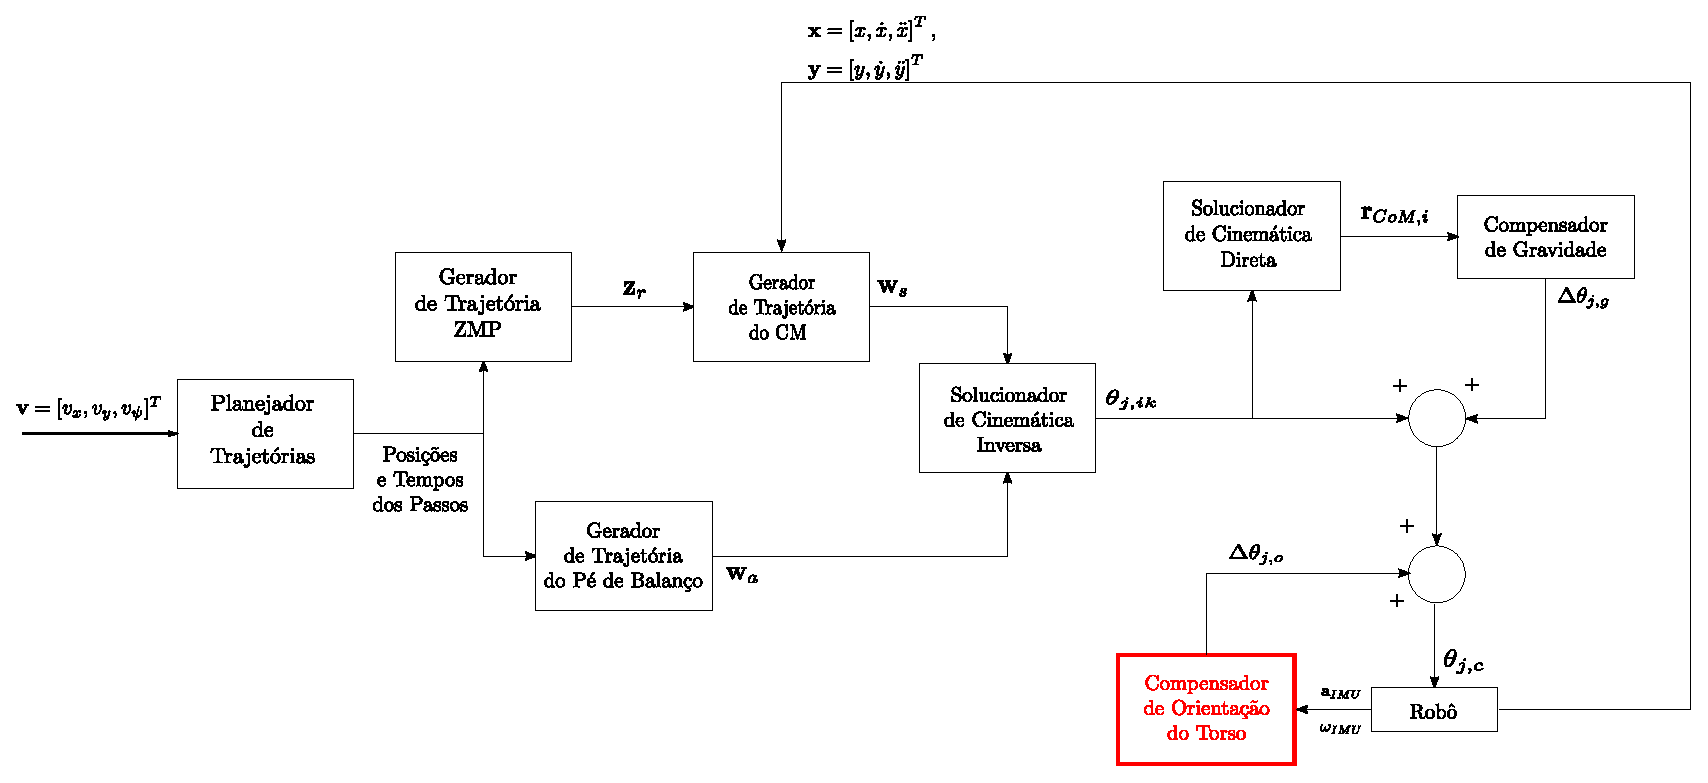
\includegraphics[angle=90, height = 0.9\vsize]{figures/walking_engine_overview.eps}
\caption{Visão geral do controle de caminhada.}
\label{fig:visao_geral}
\end{figure} 

Escolhe-se um controlador P+V e não um PD de modo a evitar amplificação de ruído por meio da derivação das estimativas de ângulo. Utilizam-se, então, as medidas de velocidade angular do girômetro. O controlador comanda o deslocamento de posição como:
\begin{align}
\Delta \theta_{hr,o} = - \left[ K_{p,hr} \left( \phi_d - \phi \right) - K_{v,hr} p \right], \\
\Delta \theta_{ar,o} = - \left[ K_{p,ar} \left( \phi_d - \phi \right) - K_{v,ar} p \right], \\
\Delta \theta_{hp,o} = - \left[ K_{p,hp} \left( \theta_d - \theta \right) - K_{v,hp} q \right], \\
\Delta \theta_{kp,o} = - \left[ K_{p,kp} \left( \theta_d - \theta \right) - K_{v,kp} q \right], \\
\Delta \theta_{ap,o} = - \left[ K_{p,ap} \left( \theta_d - \theta \right) - K_{v,ap} q \right],
\end{align}
em que \( \phi_d \) e \( \theta_d \) são ângulos desejados de rolamento e arfagem, respectivamente; \( \phi \) e \( \theta \) são ângulos atuais de rolamento e arfagem, respectivamente; \( p \) e \( q \) são velocidades angulares de rolamento e arfagem, respectivamente; os índices \( hr \), \( ar \), \( hp \), \( kp \) e \( ap \) referem-se a coxa-rolamento (\textit{hip-roll}, em inglês), calcanhar-rolamento (\textit{ankle-roll}, em inglês), coxa-arfagem (\textit{hip-pitch}, em inglês), joelho-arfagem (\textit{knee-pitch}, em inglês) e calcanhar-arfagem (\textit{ankle-pitch}, em inglês), respectivamente; \( K_{p,*} \) e \( K_{v,*} \) representam ganhos proporcionais e derivativos de cada junta, respectivamente; finalmente, \( \Delta \theta_{*,o} \) representa o comando de deslocamento (\emph{offset}) de cada junta.

Vale ressaltar que, para determinar os ganhos, lineariza-se o modelo não linear das equações do manipulador em torno de uma postura nominal (robô com velocidade zero no meio da fase de duplo suporte) \cite{tesemarcos}. A linearização é realizada pelo método de pequenos sinais \cite{franklin2013}. 

Esta modelagem é especialmente útil, visto que o robô humanoide pode ser considerado um manipulador completamente atuado se seu \textit{zero moment point} (ZMP) estiver dentro do polígono de suporte. Neste caso, considera-se que o pé do robô está preso no solo \cite{vukobratovic2004}. O ZMP é um conceito popular na literatura de caminhada, sendo o ponto no qual pode-se considerar que as forças de reação devem atuar para equilibrar o mecanismo bípede \cite{vukobratovic2004}. Quando o ZMP está dentro do polígono de suporte, este coincide com o centro de pressão da base.

Nota-se que os critérios de estabilidade utilizados mais corriqueiramente, como o critério do ZMP dentro do polígono de suporte, tratam da estabilidade local da caminhada, isto é, observa-se as condições de estabilidade para o estado atual do robô a cada passo, não para a caminhada como um todo. O fato da análise de estabilidade ser tratada localmente tornam os critérios estabelecidos restritivos, produzindo um movimento de caminhada muito aquém do melhor movimento quanto ao aproveitamento energético. Para comparação, estima-se que o robô ASIMO utiliza 10 vezes mais energia que um ser humano para caminhar \cite{tedrake2005}.

Como exposto, consideram-se dois manipuladores robóticos desacoplados, um para o plano sagital (arfagem) e outro para o plano coronal (rolamento). A Figura \ref{fig:manipuladores} mostra como decorre-se a estruturação dos dois manipuladores, em que tem-se como bases os pés de suporte. É projetado um controlador SISO para cada junta de modo a respeitar restrições de interesse (banda passante e margem de fase) com auxílio de um algoritmo de otimização Nelder-Mead (da função fminsearch do MATLAB). 

\begin{figure}
\centering
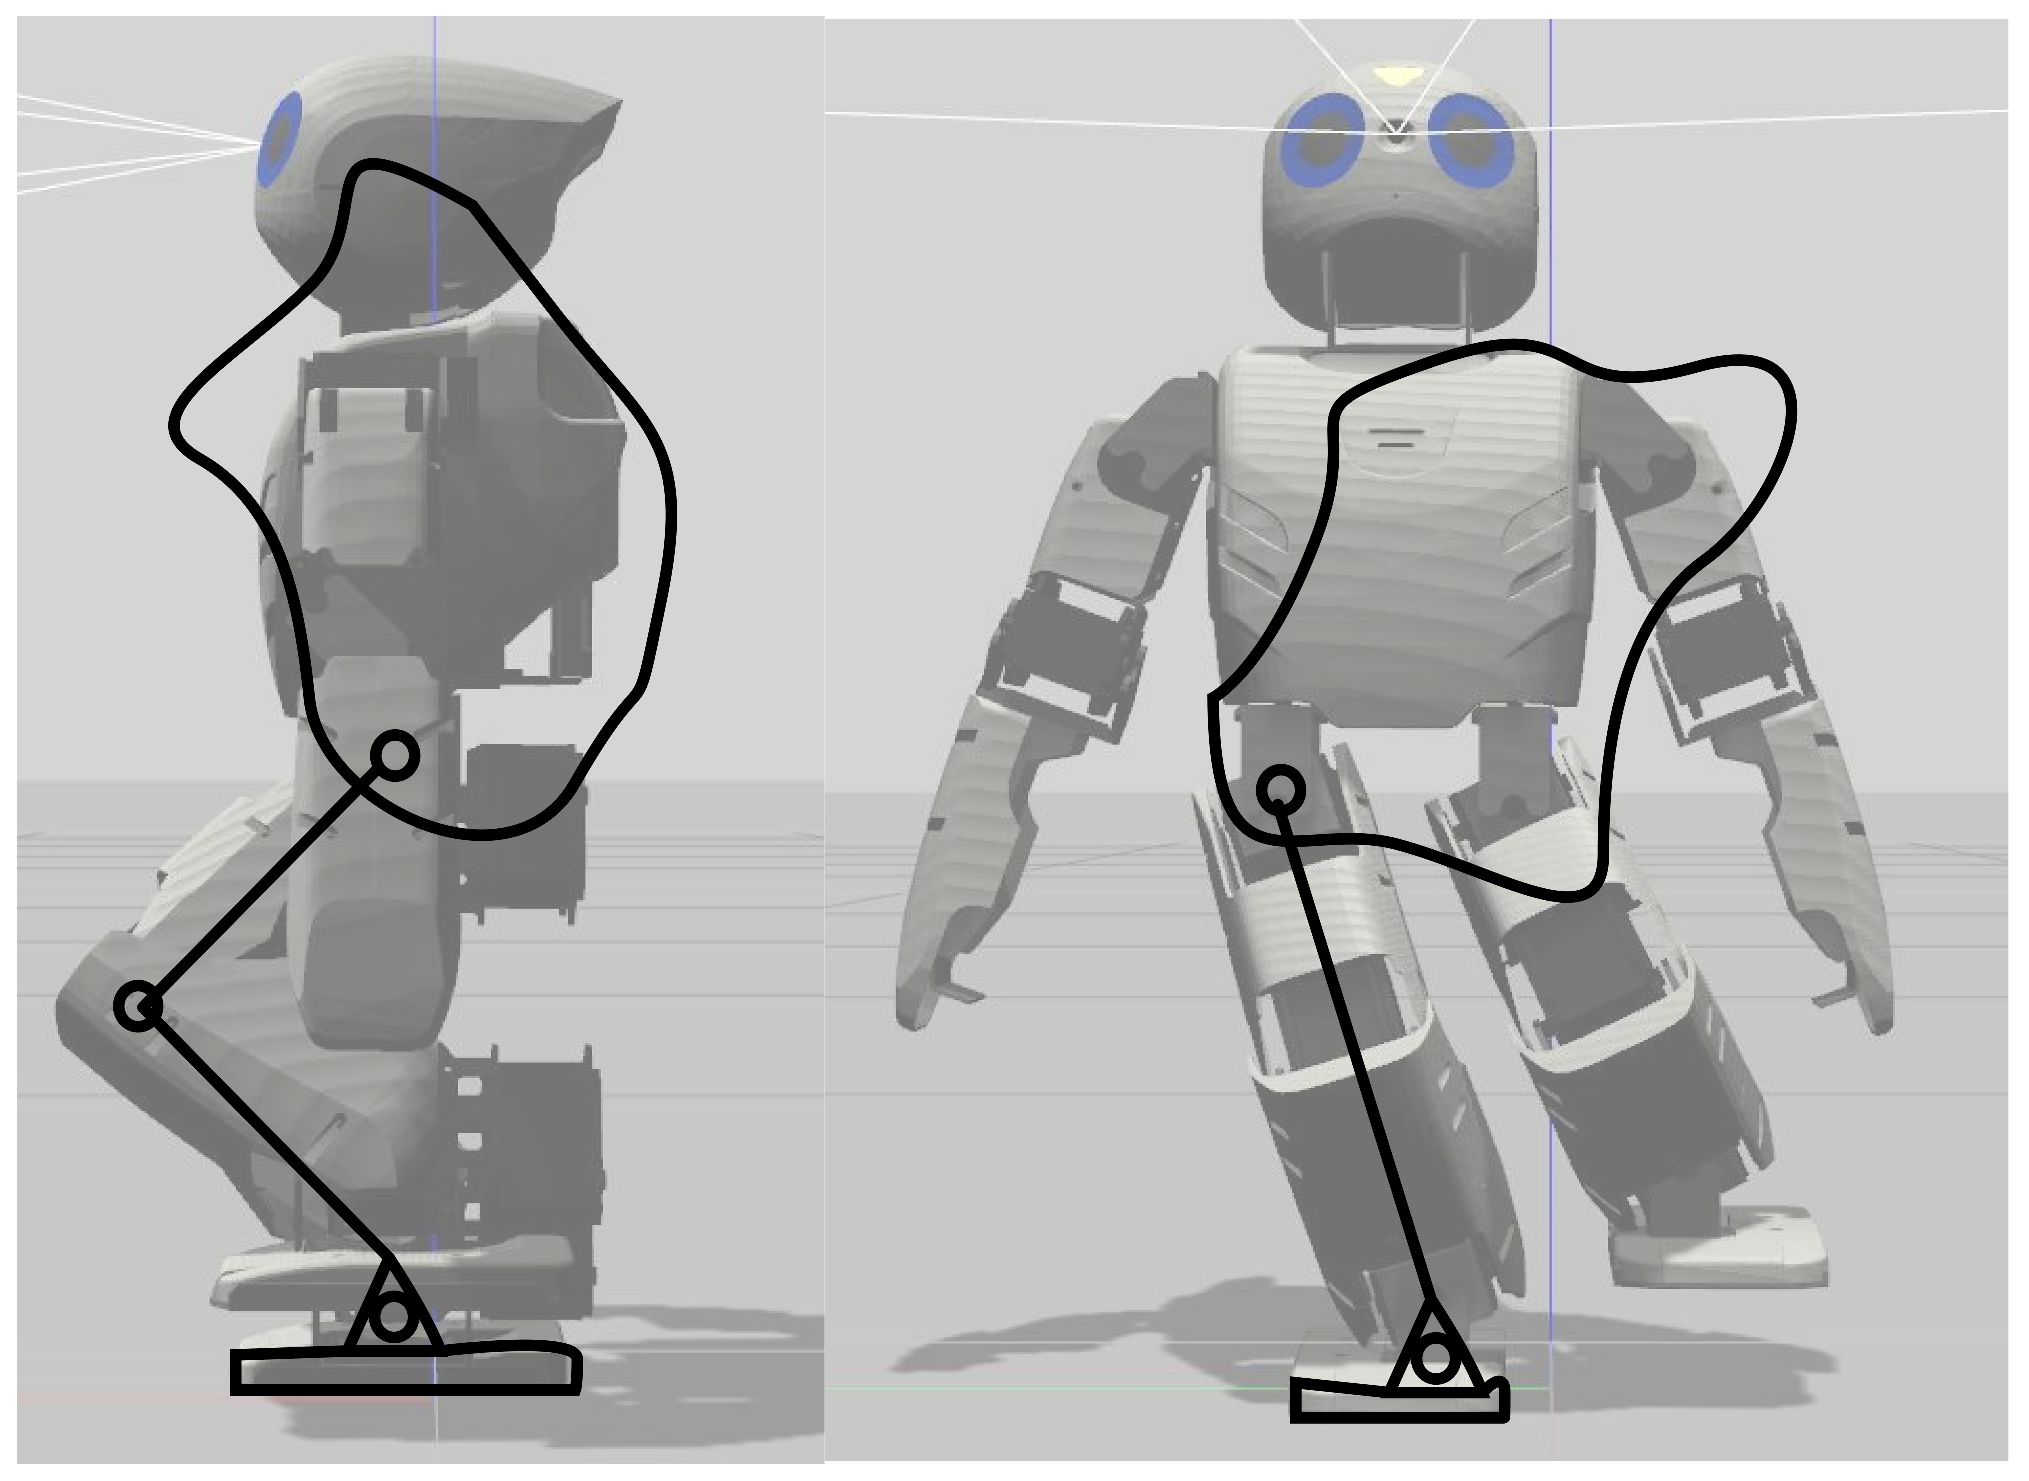
\includegraphics[width=0.5\linewidth]{figures/robo_simplificado.eps}
\caption{Simplificação do robô para manipuladores no plano sagital (esquerda) e coronal (direita).}
\label{fig:manipuladores}
\end{figure}

No desenvolvimento implementado pelo LAB-SCA em seu projeto de robôs humanoide, a interface da obtenção de parâmetros até a implementação dos ganhos \( K_{p,*} \) e \( K_{v,*} \) projetados, tem-se a interface de diferentes ferramentas. Obtém-se parâmetros a partir do modelo em CAD do robô e de medições do próprio robô físico. O modelo de dinâmica do robô e a malha de controle final completa é implementada em linguagem C++. Como mencionado, a determinação dos ganhos é feita em MATLAB. Na análise entre essas diferentes camadas de ajuste da malha de controle relacionada à compensação de orientação de torso, observaram-se algumas melhorias a serem realizadas no código da equipe.

\subsection{Reestruturação na obtenção de parâmetros}

A primeira etapa para a construção do modelo do robô humanoide é o correto ajuste de parâmetros fundamentais do robô. Para isso, utilizam-se parâmetros disponíveis a partir da montagem em CAD da mecânica do robô, como a massa, o centro de massa e o tensor de inércia de cada subsistema do robô. Outros parâmetros, como a massa total do robô, são retirados diretamente pela medição do robô físico ou de parâmetros do modelo dos atuadores. Para cada modelo de robô constrói-se uma struct dos parâmetros. 

Com a struct dos parâmetros para cada robô, adequa-se os parâmetros num sistema de coordenadas (S.C.) novo, com relação a uma origem. Esta origem pode ser o próprio centro de massa ou outro ponto de interesse fixo, sendo este último mais vantajoso pois o centro de massa muda constantemente no espaço de acordo com o movimento do robô. O método a realizar estas transformações é feito pela equipe no MATLAB, pois extrai informações uteis tanto para o código em C++ como para o modelo de simulação em Gazebo \cite{1389727}. 

Durante o estudo do código para otimização, porém, notou-se que a forma que esta etapa foi implementada era de baixa manutenibilidade. Extraía-se as informações da estrutura de parâmetros do MATLAB e estas eram colocadas no código C++ de forma \textit{hard coded}, ou seja, repetia-se a escrita dos parâmetros do robô, agora transformadas para um novo sistema de coordenadas, no código em C++ do modelo do robô.

De modo a corrigir este problema, implementou-se a interface automática entre a estrutura de parâmetros construída no MATLAB e o modelo do robô no código principal em C++ por meio de uma árvore de parâmetros em arquivo JSON. Assim, os parâmetros gerais do robô são passados apenas uma vez a um script no MATLAB e ao carregar os parâmetros para a simulação em gazebo, também constrói-se um arquivo JSON que é lido pelo código principal em C++. 

Com isto, a estrutura do código como um todo ficou mais modularizada e menos propícia a erros na escrita dos parâmetros. No MATLAB utilizou-se a função \textit{jsonencode} e, no C++, a biblioteca \textit{Boost} \cite{boost}. Um diagrama esquematizado do antes e depois da estrutura de obtenção dos parâmetros é apresentada na Figura \ref{fig:TEO_1}, em que destaca-se a utilização do arquivo JSON para evitar uma trilha de código \textit{hard coded}.

\begin{figure}
    \centering
    
    \subfloat[Sem interface de arquivo JSON.]{
    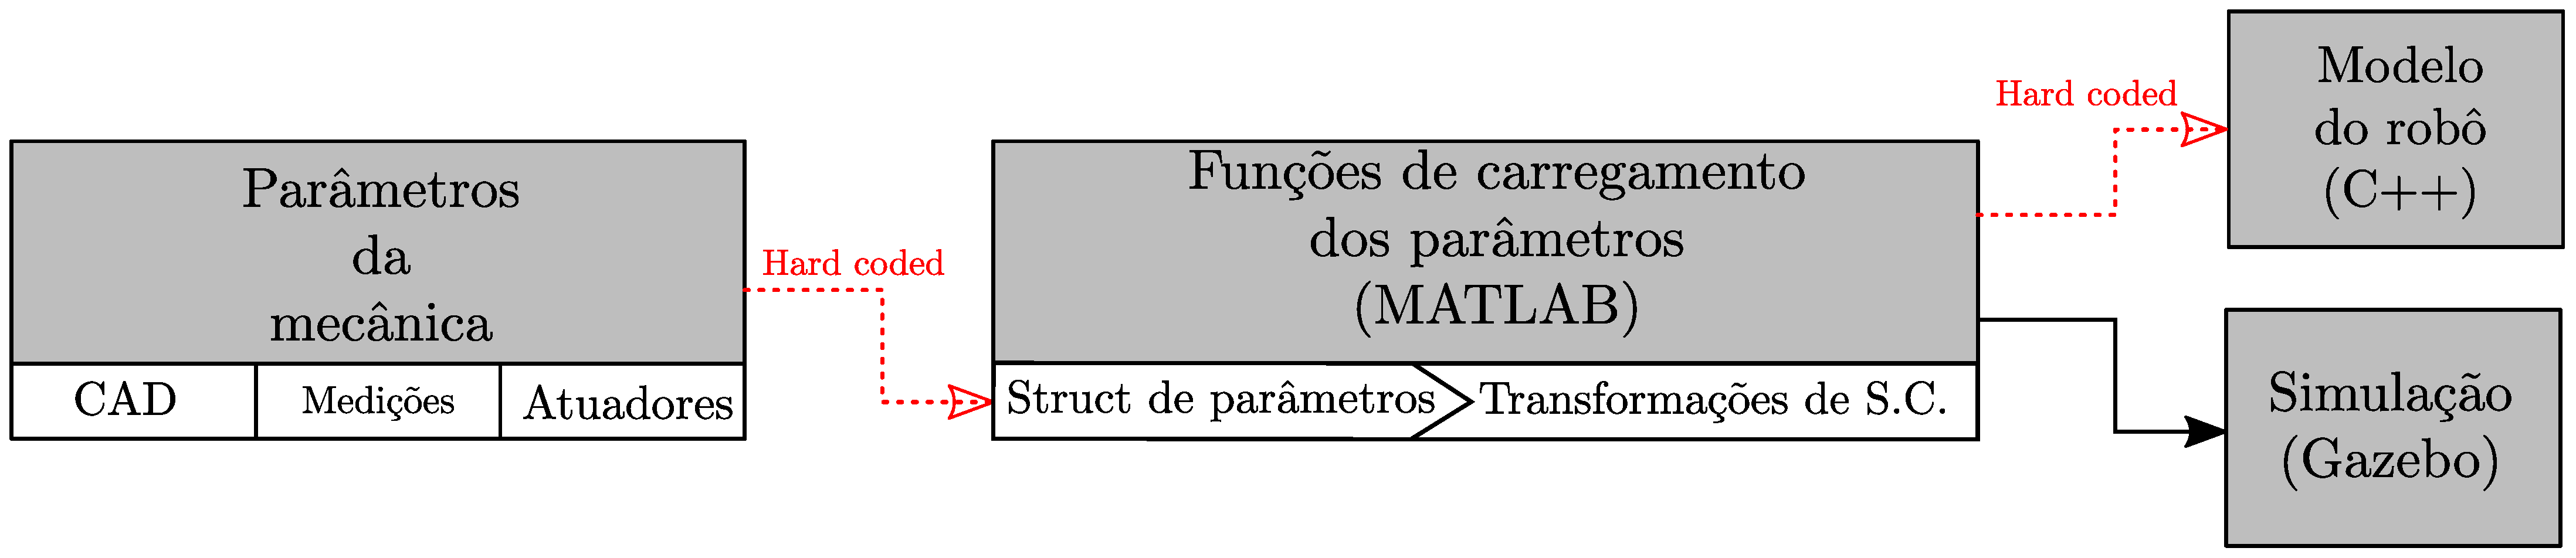
\includegraphics[clip,width=0.8\linewidth]{figures/esquema_interface.eps}
    }
    
    \subfloat[Com interface por JSON implementada.]{
    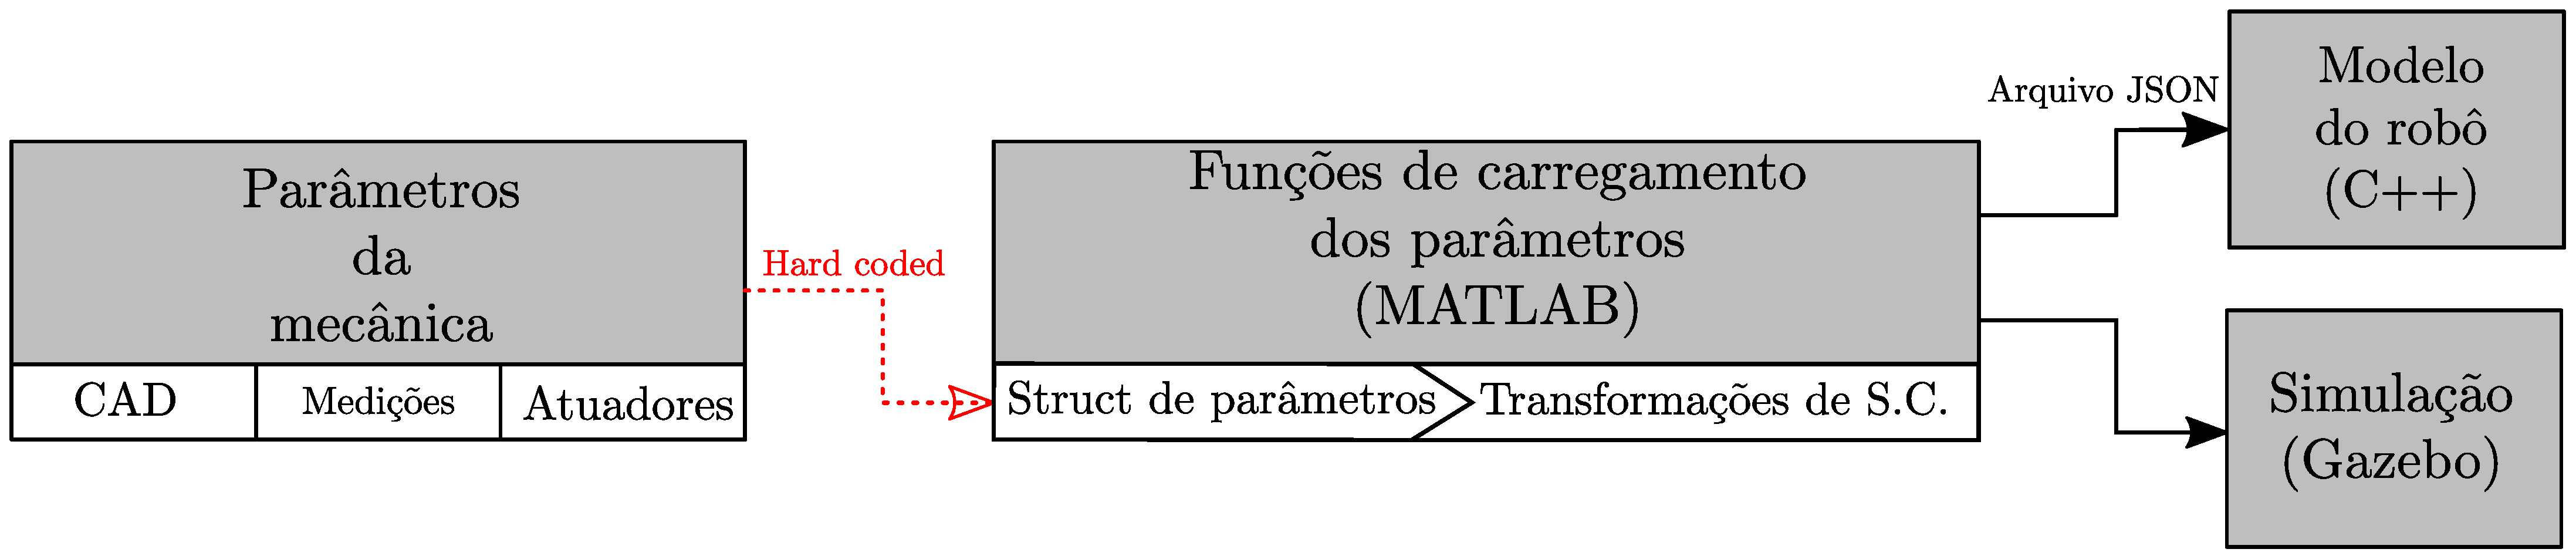
\includegraphics[clip,width=0.8\linewidth]{figures/esquema_interface_corrigido.eps}
    }
    
    \caption{Interface do carregamento e transformação dos parâmetros do robô.}
    \label{fig:TEO_1}
\end{figure}

\subsection{Plano sagital: projeto de ganhos dos controladores} \label{subsec:sagital}

\begin{figure}
\centering
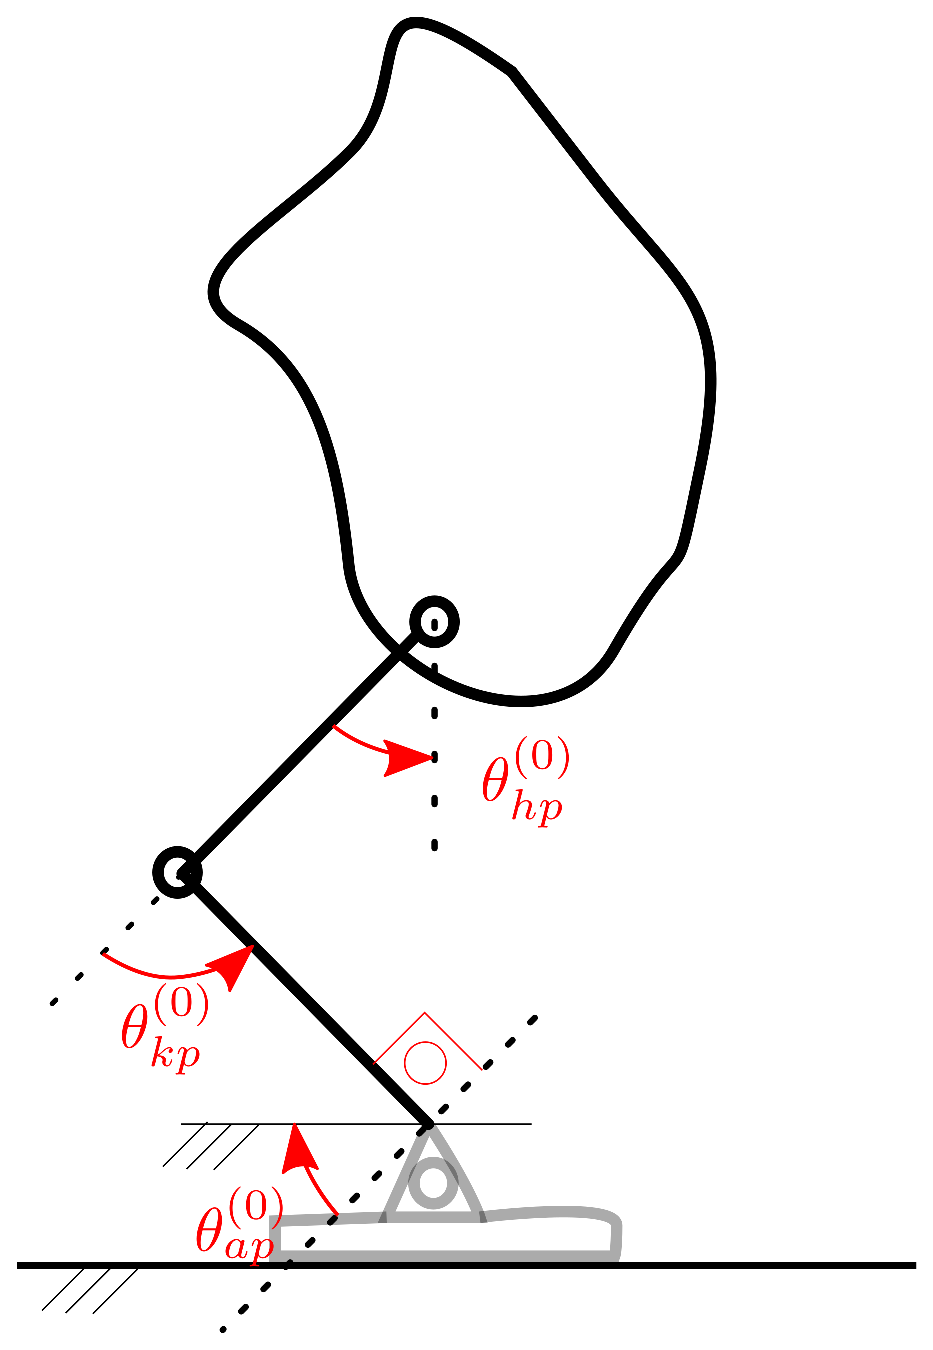
\includegraphics[width=0.4\linewidth]{figures/sagital.eps}
\caption{Representação em manipulador do plano sagital do robô humanoide.}
\label{fig:sagital}
\end{figure}

A Figura \ref{fig:sagital} mostra os ângulos base para os ângulos de arfagem do plano sagital $\theta^{(0)}_{*p}$, em que $*$ podem ser os subscritos $a$, $k$ e $h$, que representam, respectivamente, a junta do tornozelo, junta do joelho e $h$, junta do quadril \cite{tesemarcosmestr}. %Além disso, vale destacar que a linearização da equação do manipulador é feita com relação a pequenas variações destes ângulos marcados na Figura \ref{fig:sagital} (a referência para a posição base sendo o robô com velocidade nula e no meio da fase de duplo suporte).

A interface para o projeto de ganhos era iniciada a partir do modelo do robô construído no código C++. Escolhe-se a construção do modelo desta forma, pois nesta etapa facilitam-se as operações de transformação para posições de interesse e permitem a construção de modelos particulares para cada unidade de robô com suas particularidades, não apenas iterando por modelo ou geração de robô. 

Parte-se do modelo do robô em posição de T, isto é, braços completamente abertos, pernas retas e estendidas. Utilizando as bibliotecas desenvolvidas em C++ pelo laboratório LAB-SCA, são feitas as transformações do modelo para obter-se uma representação da posição assumida como padrão para o controle. 

Com esta posição, calculam-se o modelo de manipulador do plano sagital (pêndulo invertido de três elos), supondo que:
\begin{itemize}
\item Uma das pernas é assumida como pé de suporte no movimento de caminhada;
%\item A base do robô é posicionada de modo que a linha do servo do quadril com o torso sempre é vertical, o que implica :
%\begin{equation}
%\theta_{ap} + \theta_{kp} + \theta_{hp} = 0;
%\end{equation}
\item Perna e coxa constituem os dois primeiros elos do manipulador;
\item O restante do corpo do robô e o pé flutuante constituem o terceiro elo do manipulador.
\end{itemize}

Com este modelo, obtém-se do código C++ os vetores, massas e inércias dos elos descritos, formando a cadeia cinemática para o modelo. 

Com isso, é possível construir, no ambiente do MATLAB, o modelo dinâmico, aplicando a equação do manipulador:
\begin{equation}
\label{eq:dinamica}
\mathbf{B(q)} \ddot{\mathbf{q}} + \mathbf{C}(\mathbf{q}, \dot{\mathbf{q}}) \dot{\mathbf{q}} + \mathbf{g(q)} = \boldsymbol{\mathcal{T}},
\end{equation}
em que $\mathbf{q}$ é o vetor de estado dos ângulos no plano sagital, $\boldsymbol{\mathcal{T}}$ é o torque de entrada no sistema e as matrizes $\mathbf{B(q)}$, $\mathbf{C}(\mathbf{q}, \dot{\mathbf{q}})$ e $\mathbf{g(q)}$ representam, respectivamente, a matriz de inércia, efeito coriolis e gravidade da equação do manipulador \cite{10.5555/1965405}, obtidas com auxílio dos valores para a cadeia cinemática. 

Obtendo o modelo dinâmico, lineariza-se o sistema como já discutido, sendo o cálculo das matrizes jacobianas do sistema feito com o auxílio do pacote de matemática simbólica do MATLAB. Ademais, com as restrições para os servos bem conhecidas, constrói-se uma função custo e obtém-se os ganhos da otimização (ver Seção 4 do relatório parcial \cite{parcial}). Os ganhos da malha P+V do plano sagital eram, então, colocados num arquivo de configuração e serviam de entrada para o código do controle do robô, em C++.

O modelo implementado, porém, continha problemas na interface construída, algumas das quais foram corrigidas, como:
\begin{enumerate}[\textbf{P.1.}]
\item O código de Projeto de controladores sagital era feito num \emph(script) que precisava de variáveis no \textit{workspace} de dois scripts auxiliares referentes à construção do modelo dinâmico, os quais precisavam ser chamados manualmente em uma ordem específica.\\
\textbf{Solução:} Isolamento dos scripts auxiliares em funções, com o script de Projeto de controladores chamando as funções.
\end{enumerate}
\begin{enumerate}[\textbf{P.2.}]
\item O conjunto das funções era feito sem levar em consideração diferentes modelos e gerações de robôs, de modo que os ganhos projetados não levavam em consideração as individualidades do robô.\\
\textbf{Solução:} Ajuste para funcionamento do código com entrada do usuário para qual geração do humanoide pretendia-se o cálculo dos ganhos.
\end{enumerate} 
Foi notado mais uma melhoria a ser aplicada, que ainda não foi feita:
\begin{enumerate}[\textbf{P.3.}]
\item A passagem de cadeia cinemática do C++ é feita \textit{hard coded}, ou seja, escreve-se diretamente no script MATLAB os valores obtidos em C++ para os elos do manipulador.\\
\textbf{Solução a ser implementada:} fazer o código de projeto de controladores sagital rodar o binário do C++ que constrói a cadeia cinemática e obter os parâmetros para a versão mais recente do projeto.
\end{enumerate} 


\subsection{Plano coronal: projeto de ganhos dos controladores}

A Figura \ref{fig:coronal} mostra os ângulos base para os ângulos de rolamento do plano coronal. Destaca-se que para o manipulador coronal, no laboratório LAB-SCA, utilizavam-se ganhos \( K_{p,ar} \), \( K_{v,ar} \), \( K_{p,hr} \) e \( K_{v,hr} \) ajustados empiricamente. Desse modo, construiu-se um programa análogo ao mencionado na Subseção \ref{subsec:sagital}, já implementando as melhorias aos problemas P.1 e P.2.

\begin{figure}
\centering
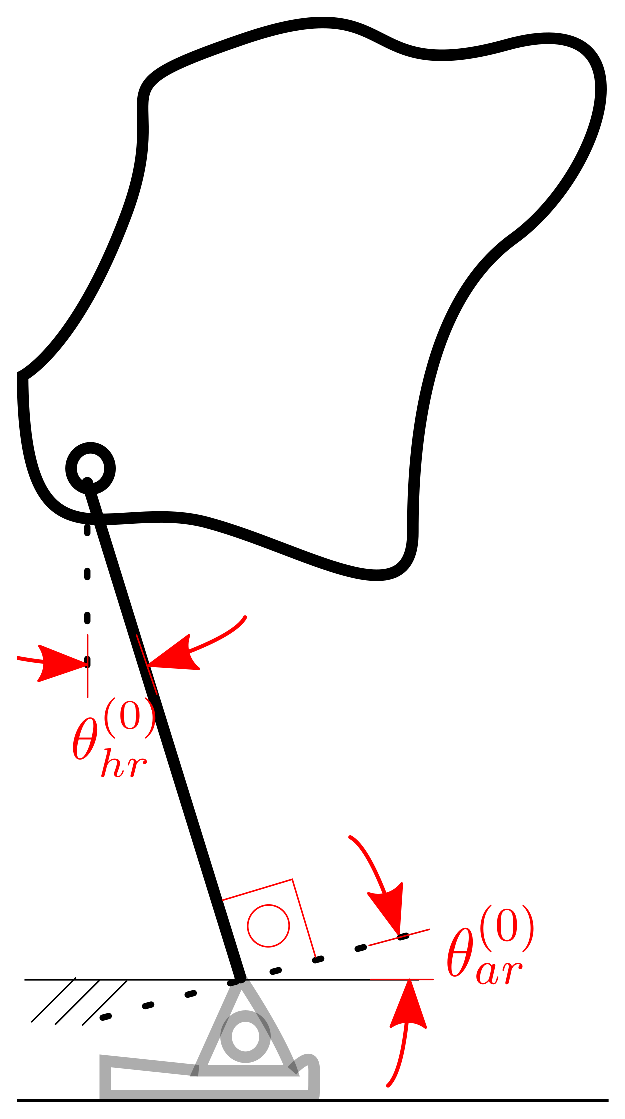
\includegraphics[width=0.3\linewidth]{figures/coronal.eps}
\caption{Representação em manipulador do plano coronal do robô humanoide.}
\label{fig:coronal}
\end{figure}

Um diagrama expondo a interface para projeto dos ganhos de controladores como eram feitos anteriormente e como devem vir a ser implementados é mostrado na Figura \ref{fig:ganhos}. Destaca-se que a solução ao trecho \textit{hard coded} ainda deve ser implementada. Ajustes propostos como um todo permitem maior modularidade e diminui-se consideravelmente a chance de erros no projeto dos ganhos. Considerando, por exemplo, possíveis modificações da mecânica do robô, no modo implementado inicialmente, da Figura \ref{fig:ganhos}.a), deveria-se executar o modelo do robô em C++ e reescrever no MATLAB a nova cadeia cinemática, enquanto com as melhorias propostas, da Figura \ref{fig:ganhos}.b), essas alterações seriam feitas em uma camada inferior (diagrama da Figura \ref{fig:TEO_1}).

\begin{figure}
    \centering
    
    \subfloat[Interface inicial.]{
    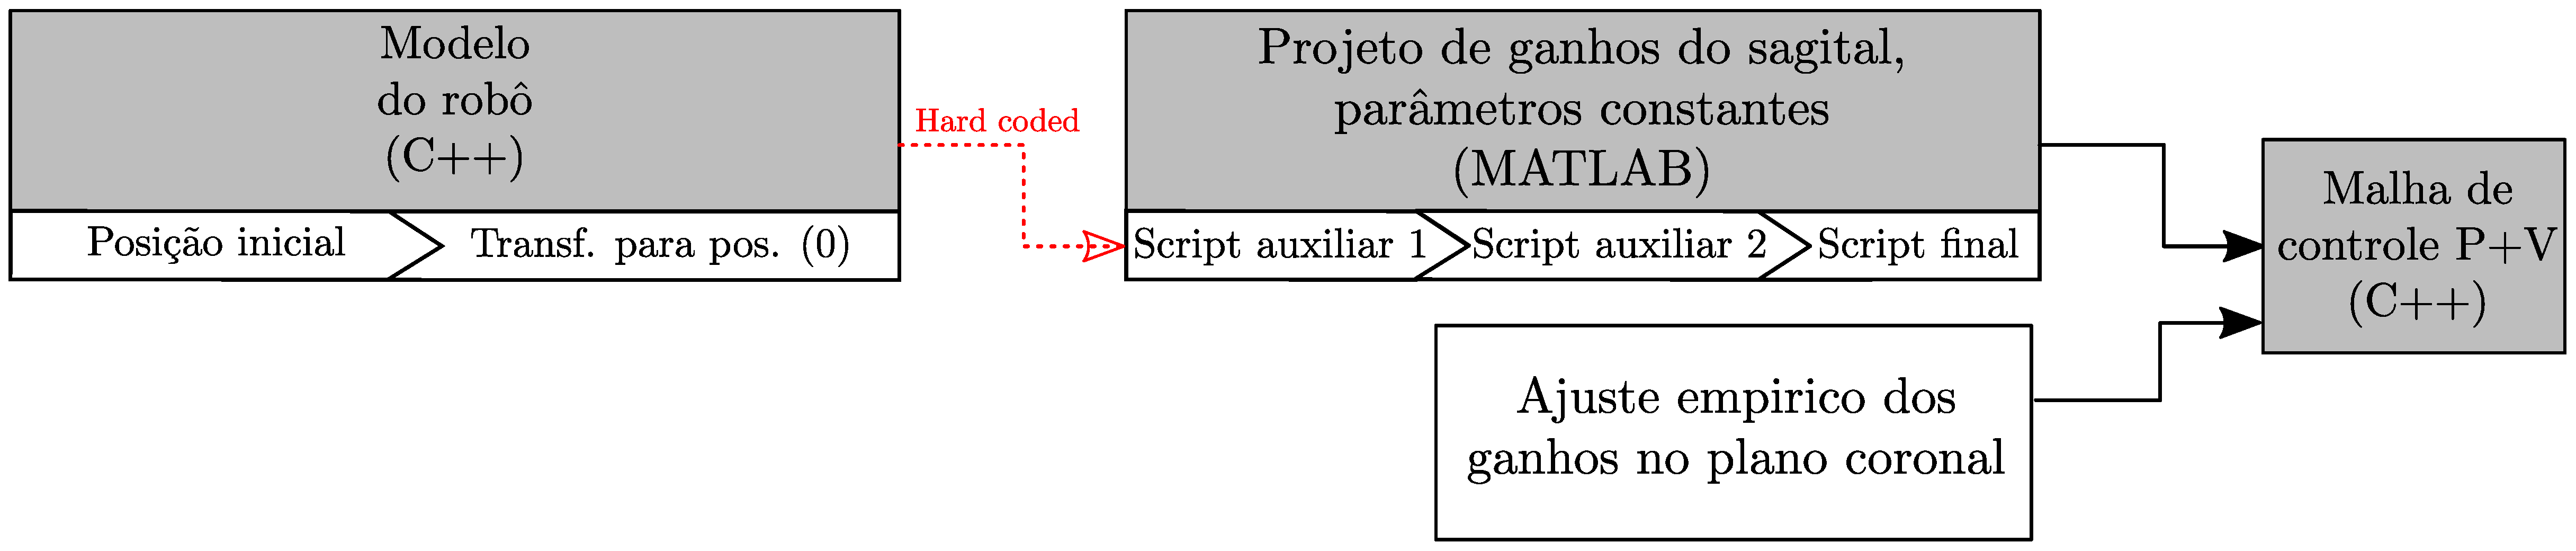
\includegraphics[clip,width=0.8\linewidth]{figures/esquema_projeto_ganhos.eps}
    }
    
    \subfloat[Interface proposta com melhorias.]{
    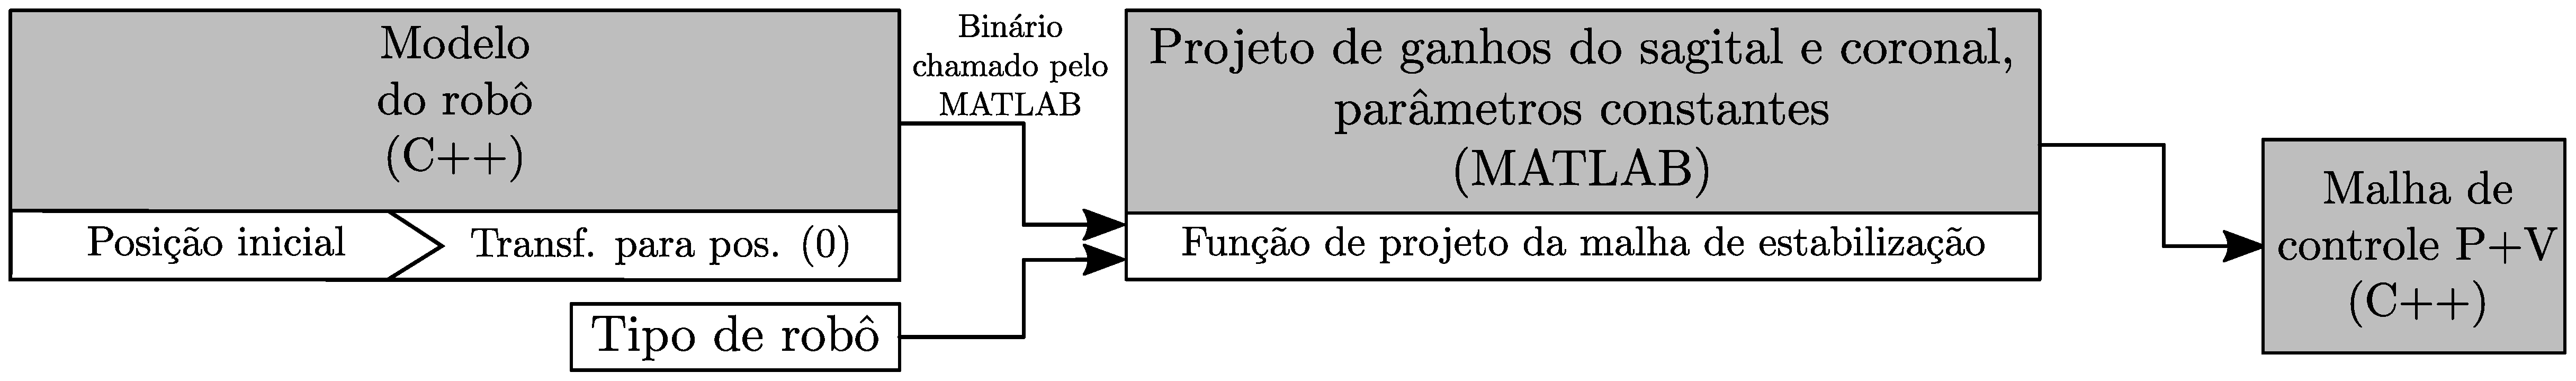
\includegraphics[clip,width=0.8\linewidth]{figures/esquema_projeto_ganhos_corrigido.eps}
    }
    
    \caption{Interface do projeto dos ganhos dos controladores.}
    \label{fig:ganhos}
\end{figure}

\section{Conclusão e trabalhos futuros}

O trabalho desenvolvido foi proveitoso em identificar os principais pontos a serem otimizados na interface do código de robô humanoide implementado pelo laboratório LAB-SCA. Destacam-se as melhorias já aplicadas e os modelos de interação entre plataformas diferentes com o mínimo de uso de códigos \textit{hard coded} (ver Figuras \ref{fig:TEO_1} e \ref{fig:ganhos}).

Destaca-se, ainda, do plano inicial da iniciação científica (ver Seção \ref{sec:plano}), que o item G teve sua atuação impactada diretamente pela pandemia do novo coronavírus, com a impossibilidade de acesso à estrutura física do LAB-SCA e, por conseguinte, dos robôs. O item H do planejamento inicial, por sua vez, foi parcialmente afetado, visto que a comparação do desempenho da obtenção dos ganhos não foi testada.

Vale ressaltar, por fim, que se esperam melhorias limitadas com o ajuste dos ganhos, visto que a implementação descrita, como um todo, é robusta e consideravelmente conservadora. Isso se deve aos critérios exigidos na modelagem da caminhada de humanoide, os quais são altamente restritivos quanto à estabilidade, como mencionado na Seção \ref{sec:estab}. 

Para trabalhos futuros, planejam-se aperfeiçoar as melhorias mencionadas na estrutura do código, bem como o estudo de ferramentas de simulação que considerem o uso do modelo de manipulador completo nos termos de primeira ordem na redução dos motores, como discutido no desenvolvimento do modelo do manipulador no relatório parcial da iniciação científica \cite{parcial}.

Com os modelos estudados e aperfeiçoados, além de pontos levantados como pouco mencionados na literatura de robôs humanoide, pretende-se publicar resultados deste trabalho nos seguintes congressos:
\begin{itemize}
\item Congresso brasileiro de automática, CBA;
\item Latin America Robotics Symposium, LARS;
\item International congress of mechanical engineering, COBEM.
\end{itemize}

Vale ressaltar, ainda, que o tema desenvolvido na iniciação científica serviu de proposta para a entrada do beneficiário no programa de mestrado na graduação (PMG) do Instituto Tecnológico de Aeronáutica, no programa de Pós-Graduação em Eng. Eletrônica e Computação (EEC).

No mestrado, pretende-se desenvolver um controlador preditivo de posição do movimento de caminhada, assumindo as hipóteses de posição do ZMP como restrições ao controlador. Além disso, para a implementação deste controlador, pretende-se partir da construção de um estimador de estados, incluindo a posição, orientação, velocidade linear e velocidade angular a partir do conjunto de dados da unidade inercial e posição dos membros.

%Construção do estimador de estados do robô (posição, orientação, velocidade linear e velocidade angular) a partir do conjunto de dados da UMI (aceleração linear e velocidade angular) e posição dos membros (calculadas a partir das posições das juntas e do modelo cinemático do robô).
%Calcular, a partir dos estados estimados, a posição do ZMP e o modelo de controle como um todo. Linearizar o sistema dinâmico de modo a utilizá-lo no controlador.
%Desenvolver um controlador que aproveite todos os estados estimados para estabilização da caminhada.
%Adição de restrições do movimento do ZMP no controlador por meio de controle preditivo.



%\section{Referências}

\newpage
\printbibliography
\end{document}